\section{Hand Motion Dimensionality and PCA}

At the core of our technique is the assumption that hand motion is relatively low-dimensional.  Even though a full resolution skeleton of the hand can have several dozen degrees of freedom (DOF), many of the DOFs of the hand show correlations, so that the inherent dimensionality of the hand motions is much lower ~\cite{SanFlaSoe98,BraZha04,JoeOSu09}. In our approach, PCA is used to exploit this low dimensionality as we assume that PCA will allow us to capture the important features of the whole-body hand motion in a small number of principle components.  
%Further, we assume that if we record markers that well-inform these \emph{key} principle components, we can estimate the DOFs of the whole hand.

To support these assumptions, we performed various tests to study the power of PCA for capturing the desired reduced dimensionality of hand motion. 
In Figure~1 below we show that PCA is indeed capable of reducing the dimensionality of the joint angle motion from the database, revealing low average errors for simple reconstruction with reduced numbers of components.  This figure shows erros applied to our ASL database, which represents a diverse expression of poses for the hand.  We see that PCA shows significant reduction in reconstruction error after around 10 components.  While this is larger than reported findings for finger motion, the rich full hand gestures of ASL are still well-represented with a relatively small number of components.
Similar findings are reported using a small set of components from PCA to encapsulate the motion of full-body motion~\cite{SafHodPol04} and our results here support similar observations made over hand motions.


\begin{figure}[!h]
  \centering
  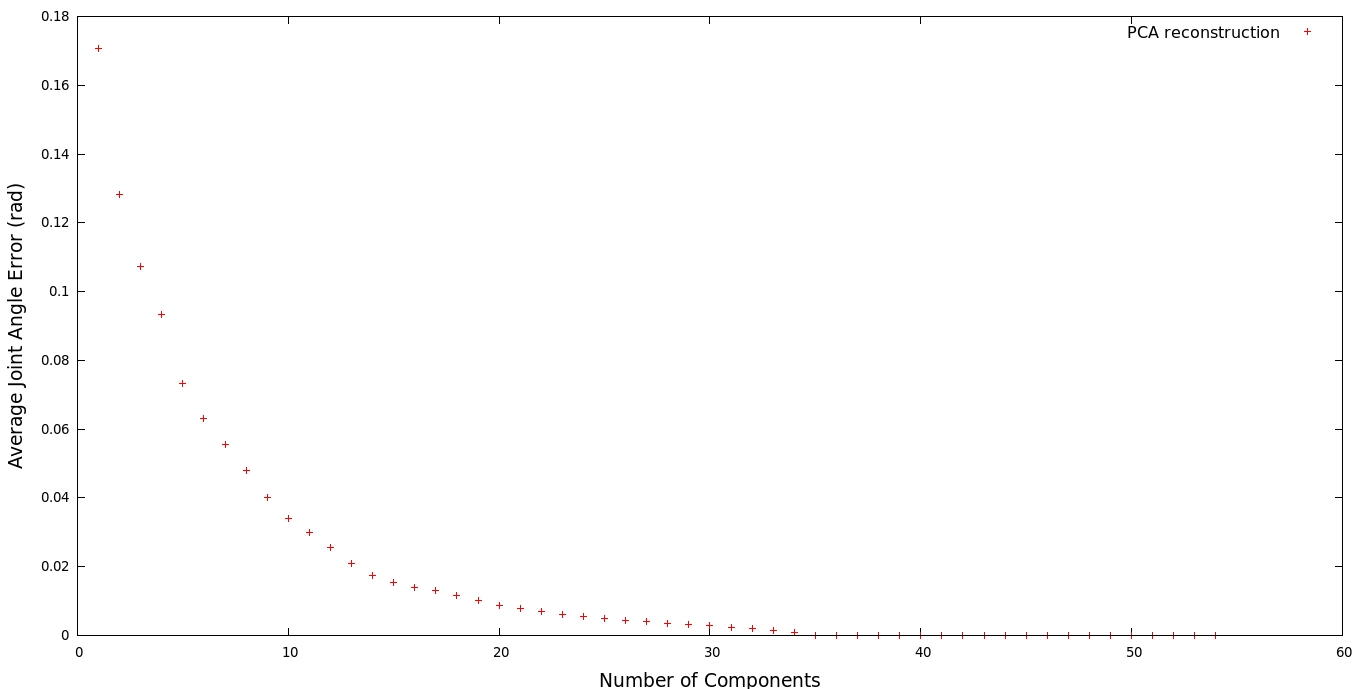
\includegraphics[width=8.3cm]{images/PCA_alphabet_reconstruct.jpg}
  \caption{{\label{fig:pcaError}}Dimensionality reduction for sign language database.  PCA is capable of using as few as ten components with relatively small average errors.}
\end{figure}

\begin{figure}[!h]
  \centering
  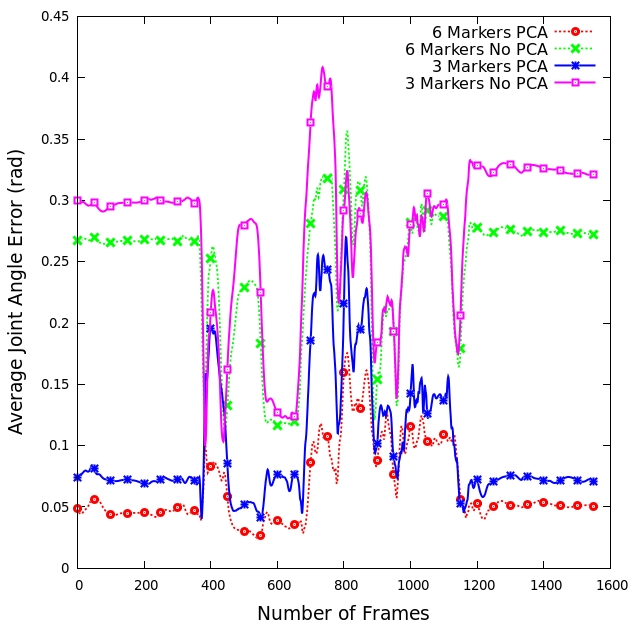
\includegraphics[width=6cm]{images/avgError_6_3_jangles_babySigns1.jpg}
  \caption{{\label{fig:avgError}} Sign language sample motion with and without PCA employed.  Note the
error for six markers without PCA is larger than that of three markers with it. }
\end{figure}

% I know this next bit is weird but the point of the section is to motivate the problem for our domain, 
% and the second figure here is really driving that home

Next, to compare the power of PCA for our particular application we experimented with two reconstruction 
methods with and without PCA. 
The details of the reconstruction appear in Section~6, however, we include the plot in Figure~2 here to support that PCA is very effective in producing higher quality hand motion.
In the figure, we clearly see the benefit of employing PCA as a go-between from markers to joint angles.
When we attempt to reconstruct without it (i.e. markers to joint angles directly) the error remains large
even as the number of markers employed to inform the hand-over process is doubled.



\begin{figure}
  \centering
%  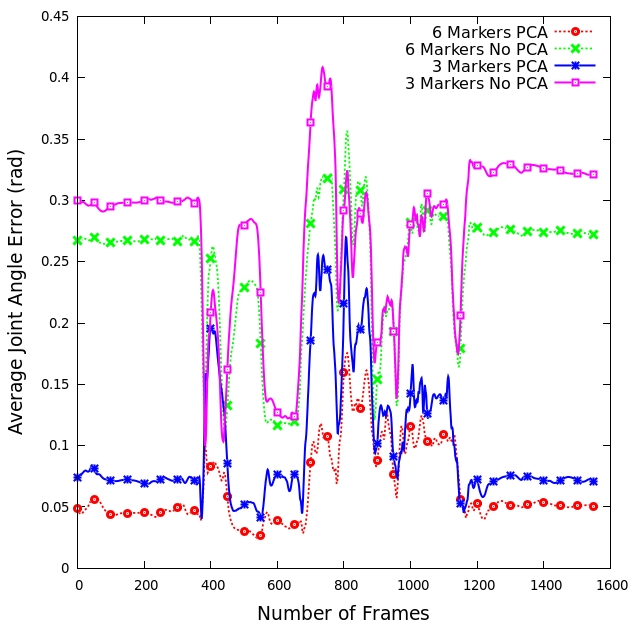
\includegraphics[height=4cm]{images/avgError_6_3_jangles_babySigns1.jpg}
 % \caption{{\label{fig:avgError}}PCA vs. Joint angles.}
\end{figure}

